\chapter{Introduction}

\section{Overview on island effects}
(TODO)

\pagebreak

\section{Transformers and the Attention Mechanism}
..
a non-recurrent architecture, called the Transformer \citep{vaswani2017attention} 
The lack of recurrence enables greater within-training-example parallelization, at the cost of quadratic complexity in the input sequence length  \citep{liu2018generating} 
..
Jurasfy book (draft new 3rd edition), ch.10 ..
\citep[ch.9-10]{jurafsky2021speech} 

..
"the terminology used to describe the Transformer, the attention is a function of a query (Q) and set of key (K) and value (V ) pairs" \citep{liu2018generating} 
multi-head self-attention of the Transformer

to reduce memory usage, limiting the dot products between Q and K
..
"projecting the tokens into the query, key, and value embeddings"
..
decoder-only vs encoder-decoder
what is an attention head? See "explorable transformers" 

\href{https://huggingface.co/exbert/?model=gpt2&modelKind=bidirectional&sentence=The%20girl%20ran%20to%20a%20local%20pub%20to%20escape%20the%20din%20of%20her%20city.&layer=0&heads=..0,1,2,3,4,5,6,7,8,9,10,11&threshold=0.7&tokenInd=null&tokenSide=null&maskInds=..&hideClsSep=true}{exbert}
..
give detailed description of each layer dimensions (eg vocab x ..)
compare bert and gpt architecture
explain output of gpt and bert
..
save the checkpoints of gpt and bert with pythorch inspect the layers
..
(from machine learning course lectures: name of "augmenting" the input ..)(..appropriate name for semantic info addition?)(LBE, linear basis expansion)(..equivalent to semantic augmentation of the input?)
..
..
schema of the self-attention mechanism (multipling on prev inputs)
(horizontal vs vertical attention?)
criticism of attention mechanism (refs)
alternative attention mechanism
attention mechanism more efficient for NLP
auto pruning of attention heads?
..
cross-entropy loss
Jurasfky 3rd ed. ch.9: "During training, the probability assigned to the correct word is used to calculate the cross-entropy loss for each item in the sequence. As with RNNs, the loss for a training sequence is the average cross-entropy loss over the entire sequence." 
(figure 9.21)
..
query, key, value


\pagebreak

\section{On the output of Gpt unidirectional language models}

The GPT architecture \citep{radford2018improving} ..
% TODO: intended meaning of the loss measure, sentence likelihood, contrast with sentence acceptability, .., ungrammatical sentences that are more likely than rarer grammatical ones, ..)
% (math formulas of Gpt output, activation functions..)

% C’è da aggiungere che la loss del modello gpt (score PenLP), usato come misura di accettabilità, è in realtà una stima globale della ..likelihood della frase (reference for this .. from gpt paper or other paper on ..transformers based language models). Ciò non corrisponde esattamente ad un giudizio di accettabilità/grammaticalità. Infatti, potrebbe darsi il caso, che una frase piuttosto comune (..) ma con un errore (sintattico, semantico, o altro) riceva una ..loss/likelihood maggiore di una frase. grammaticalmente corretta ma “rara”, o meglio, che usa un costrutto ricercato.. (es. ..).
(TODO)


..
recap: average cross entropy loss should be how the gpt2 output loss is calculated (add img with Jurafsky figures)
..check with transformers code how it's actually calculated
(calls torch CrossEntropyLoss, which "computes the cross entropy loss between input and target")


gpt forward method:

% https://www.overleaf.com/learn/latex/Code_listing
\begin{lstlisting}[language=Python]

# modeling_gpt2.py

class GPT2Model(GPT2PreTrainedModel):
    def __init__(self, config):
    	..
    def forward(
	    self,
	    input_ids=None,	
	    ..
	 ):
	 	..
	 	return BaseModelOutputWithPastAndCrossAttentions(
		 	last_hidden_state=hidden_states,
		 	past_key_values=presents,
		 	hidden_states=all_hidden_states,
		 	attentions=all_self_attentions,
		 	cross_attentions=all_cross_attentions,
	 	)

class GPT2LMHeadModel(GPT2PreTrainedModel):	

	def __init__(self, config):
		self.transformer = GPT2Model(config)
		self.lm_head = nn.Linear(
			config.n_embd, 
			config.vocab_size, bias=False
		)
	
	def forward(input_ids=None, ..	labels=None, ..):
		r"""labels (`torch.LongTensor` of shape 
		`(batch_size, sequence_length)`, *optional*):
		Labels for language modeling. Note that the labels **are shifted** inside the model, i.e. you can set
		`labels = input_ids` Indices are selected in 
		`[-100, 0, ..., config.vocab_size]` 
		All labels set to `-100` are ignored (masked), the loss is only computed for labels in `[0, ..., config.vocab_size]`
		"""
		
		transformer_outputs = self.transformer(input_ids, ..)
		hidden_states = transformer_outputs[0]  # last_hidden_state or hidden_states?
		lm_logits = self.lm_head(hidden_states)
		shift_logits = lm_logits[..., :-1, :].contiguous()
		shift_labels = labels[..., 1:].contiguous()
		
		loss_fct = CrossEntropyLoss()
		loss = loss_fct(
			shift_logits.view(-1, shift_logits.size(-1)), 
			shift_labels.view(-1)
		)
	
		return CausalLMOutputWithCrossAttentions(
			loss=loss,
			..
		)
\end{lstlisting}

% todo, clarify: cross entropy fun takes (input, target), but gpt2 calls it with (logits, labels), which are both the sentence_ids (the ids of the tokens in the sentence)

pytorch CrossEntropyLoss formula:

\begin{lstlisting}
	
class CrossEntropyLoss(_WeightedLoss):
	def forward(self, input: Tensor, target: Tensor) -> Tensor:
		return F.cross_entropy(input, target, ..)
		
		lm_logits = self.lm_head(hidden_states)
\end{lstlisting}

usage:
\begin{lstlisting}
model_output = model(
sentence_ids_in_batch_as_tensor,
labels=sentence_ids_in_batch_as_tensor,
)
loss = model_output.loss
\end{lstlisting}

From the pytorch cross entropy documentation, about the two parameters input and labels:

"The input is expected to contain raw, unnormalized scores for each class. input has to be a Tensor of size (C)(C) for unbatched input, (minibatch, C)(minibatch,C) "



\pagebreak

\section{On the output of BERT-like bidirectional language models}
(TODO)
% On the use of the Softmax, the logistic function (or possibly a probability measure based on the logistic function, but dividing all values for the total sum)

\pagebreak

\section{Sentence acceptability estimates}

The Formula for the sentence acceptability estimates \( LP, PenLP \) from \citet{lau2020furiously} are:

\subsection{Softmax, logistic function, and other activation functions applied to the models' output}
\label{sec:softmax}
We calculated the LP and PenLP measures taking as a basis the models' outputs after the softmax activation function applied to the last layer. 

As an alternative, for BERT-based models, we also experimented with using a logistic function rather then the softmax. We called the resulting scores LP-L and PenLP-L to distinguish them from the softmax based ones. Note that with the logistic function, for the masked word prediction scores, we still obtain a value between [0, 1] for each word in the model vocabulary, but this is not a probability since the sum of all the values is greater than one.
% TODO: consider normalizing so the sum is equal to 1?.
% see paper by .. , in which, instead of the top k scores, for predictions they use the ..top-p, that is, the top words that in aggregate reach a probability threshold p. NB: the purpose of such measure is for text generation, and it doesn't seem applyable to the present study (sentence scoring).

The formulas for LP and PenLP (taken from \citep{lau2020furiously})are:

\begin{displaymath}
	LP = \log P(s)
\end{displaymath}
\begin{displaymath}
	PenLP = \frac{LP}{((5+|s|) \big/ (5+1))^\alpha}
\end{displaymath}

Where \( P(s) \) is the probability of the sentence \( s \). The PenLP divides the \( LP \) estimate by a penalty term which depends on the sentence lenght \( |s| \), measured in number of tokens. Following \citet{lau2020furiously}, we use \( \alpha=0.8 \).

For BERT-like models, we use the estimate from \citet{lau2020furiously} of the log probability LP of a sentence s. It is estimated by masking each word in s, calculating the probability of the prediction of the masked word, and summing the log of all these probabilities:
\\ ..


\section{Research questions}

Context, lit review ..
the literature on syntactic tests.. intrinsic tests
the purpose of syntactic/linguistic fine-grained tests

research question it might ask:

..use of a factorial design
is that a complementary way to test language models?

does these tests in particular tells us something more/new/.. about ..what these models learn about language/how they learn it?

how does these tests compare to previous ones? on similar phenomena (english)
between languages (english vs italian)
in phenomena present in both english and italian vs new phenomena present in italian but not english
(some of these might not be .."research questions", but ..ways to analyse/interpret our results.. therefore belonging more to methodology than research questions)

(todo: run the english tests, using the Sprouse english datasets, seeing the accuracy results for these models (bert, roberta, gpt)

(about the tests on Bert, and the question if it's getting cues from other words in the sentence, because it's a bidirectional LM unlike gpt..)

TODO: add methodology section .. find refs on "methodology", gathering and analyzing data

explain the decision of building a manual test set
compare with blimp autogenerated test set
detail ..which factor are controlled in our example
following sentences schema from sprouse et al.



quote umberto eco at the beginning on the section on methodology
(translate it)

\subsection{ItaCola from Trotta et al. 2021}

the meaning of cross entropy (average?)
even in the case of gpt, can it be used as an estimation/approximation of sentence acceptability?
or is this problematic/a ..forzatura
only in the case of minimal pairs (in the strict sense of differing by 1 word), ..
otherwise the ..cross entropy loss ..might mean, likelihood, sentence likelihood, and still, in natural language use, some frequenty incorrect sentences are more likely than rare ones

Trotta et al 2021 Monolingual and Cross-Lingual Acceptability Judgments with the Italian CoLA corpus

finetune the models for acceptability? (already existin italian models for this, like from Trotta et al. 2021?)
finetuning is very fast anyway 

domande per Lenci:
possibili obiezioni sui dati raccolti, il dataset creato:
differenze rispetto a paper che controllano per certi fattori, escludono certe frasi, ..ripuliscono il dataset secondo vari criteri

"An additional check was performed to manually
control for typos and transcription errors."

out contributions wrt to trotta et al 2021:
comparable number of examples (50), but for more phenomena (4 instead of 1)
difference in the wh-islands phenomena
NB in fig.1 (right) trotta et al also omit the wh islands results
problem in trotta et al for sentences with multiple phenomena
(check if some sentences in our dataset also show any of the other phenomena tagget in trotta et al)(if not, another advange of our contribution)

"The fact that classification of sentences containing only one phenomenon yields better results holds for all categories except for Questions and Auxiliary"

"Interestingly, Wh-islands violation
does not appear in the chart on the right because
this phenomenon is always accompanied with at
least another annotation"


(fine tune also for english the Bostrom models?)

"(Gao et al., 2020) shows that pre-trained LM performs worse in some tasks such
as linguistic acceptability task and natural language inference task since pre-trained LM barely saw
this data distribution." (Wang et al 2021 Entailment as few shot learner)

Alternative training tasks:
"Task reformulation: Language model is usually pre-trained with a Masked Language Modeling
(MLM) objective, which is motivated by Cloze task in (Taylor, 1953). There have been several
works reformulating few-shot learning tasks as cloze questions to reuse pre-trained LM such as
LM prompt (Jiang et al., 2020), PET (Radford et al., 2019; Schick \& Schutze, 2020a), and recent ¨
LM-BFF (Gao et al., 2020). It shows a pre-trained LM can achieve non-trivial performance with few annotated samples. There are also some other works transforming NLP tasks as generative QA tasks (Puri \& Catanzaro, 2019)."
but low performance on CoLA (possible beacuse of "different data distribution"):
"The only exception is the CoLA (the linguistic acceptability task). It
is might due to that MLM pre-trainng and entailment training did not see this type of data distribution before"

enriched training data (with supervised tasks):
"Intermediate training: The work by (Phang et al., 2018) shows that supplementing pre-trained LMs with further training on data-rich supervised tasks can obtain additional performance improvements on the GLUE benchmark."

"Linguistic competence of neural language models (LMs) has emerged as one of the core sub-fields in NLP. " "research paradigms" (Cherniavskii et al. 2022 Acceptability Judgements via Examining the Topology of Attention Maps)

A particular interest of language in AI, is that it ..measures AI models with ..different concepts ..phenomena for which some of the standard ..alghoritmic/statistical or teory of information ..metrics, approaches, .. , don't work (eg. perplexity, ..probability estimation of next word, ..)

"Prior work has demonstrated that heads
induce grammar formalisms and structural knowledge (Zhou and Zhao, 2019; Lin et al., 2019; Luo,
2021), and linguistic features motivate attention
patterns (Kovaleva et al., 2019; Clark et al., 2019)."
"Recent studies also show that certain heads can
have multiple functional roles (Pande et al., 2021)
and even perform syntactic functions for distant
languages (Ravishankar et al., 2021)."
(Cherniavskii et al. 2022)

Freezing / Frozen Layers:
"The results align with Lee et al. (2019), who discuss the performance degradation of BERT-based models depending upon the number of frozen layers." (Cherniavskii et al. 2022)

note on thesis:
our contributions are as follows:
a dataset for some specific island effects phenomena in italian
experiments
..
(as in the ItaCoLA paper)


Minimal pairs vs sentence acceptability (with CoLA)
study for lau et al is ..intermediate in comparing sentences that are not strictly minimal pairs
acceptability: absolute score
minimal pairs: relative score, compared btw two sentences
Follow study from Trotta et al, and the original CoLA paper 
also minimal pairs scoring is done with the pretrained models, while CoLA involves finetuning

"Our results identify specific syntactic features
that make sentences harder to classify, such as
long distance dependencies (What do you think I
ate?), and others that have little effect on difficulty, such as non-canonical argument structures
like passives (The book was read)." (Warstadt and Bowman Linguistic Analysis of Pretrained Sentence Encoders with Acceptability Judgments)

exemplary analysis acceptability results from the cola paper:
"Our results identify specific syntactic features
that make sentences harder to classify, such as
long distance dependencies (What do you think I
ate?), and others that have little effect on difficulty, such as non-canonical argument structures
like passives (The book was read). Furthermore,
some constructions highlight or minimize the differences between models. For example, GPT and
BERT far out perform the BiLSTM on movement
phenomena such as clefts (It is Bo that left), yet
have no advantage on sentences with adjuncts (Sue
exercises in the morning). We wish to exercise
caution in interpreting these results since it is not
clear to what extent an encoder’s failure on a particular phenomenon is due to a weakness of the
encoder rather than the training data or probing
classifier. However, this caveat applies to varying
degrees to all probing resources. In this context of
other similar linguistically informed datasets, our
analysis set addresses the critical need for a evaluation task with wide coverage of linguistic phenomena"

"Hence, unacceptable sentences in CoLA tend to
be maximally similar to acceptable sentences and
are unacceptable for a single identifiable reason."   (Warstadt and Bowman Linguistic Analysis of Pretrained Sentence Encoders with Acceptability Judgments)

on the alternative of minimal pairs:
"This task is often employed
to evaluate language models because the outputted
probabilities for a pair of minimally different sentences are directly comparable, while the output
for a single sentence cannot be taken as a measure
of acceptability without some kind of normalization (Lau et al., 2016)"

"Accordingly, CoLA, but not datasets based
solely on preferences between minimal pairs, may
be used to evaluate models’ ability to make judgments that align with both native speaker judgments and the predictions of generative theories."

note the processing that was done for CoLA and ItaCoLA, ie editing less common words by checking their occurence, respectively, in the BNC and .. (a tool .. for it), noting that we ..did not check that ..for time constraints ..

" Our large sentence encoders are limited
to 100-200 million tokens of training data, which
is within a factor of ten of the number of tokens
human learners are exposed to during language
acquisition (Hart and Risley, 1992).11 
11Hart and Risley (1992) find that children in affluent families are exposed to about 45 million tokens by age 4.
" (Warstadt et al 2019 Neural Network Acceptability Judgments)
Hart and Todd R. Risley. 1992. American
parenting of language-learning children: Persisting differences in family-child interactions
observed in natural home environments. Developmental Psychology, 28(6):1096.


"Addressing this problem will likely involve new forms of regularization to mitigate this
overfitting and, more importantly, new pretraining
strategies that can help the model better learn the fundamental ingredients of grammaticality from
unlabeled data" 

"The poor performance of our models on contrasts involving agreement (Singular/Pl and Reflexive) is surprising in light of findings by (Linzen
et al., 2016) that LSTMs can identify agreement
errors easily even without access to sub-word information. We speculate that this is due to underrepresentation of the relevant examples in CoLA.
"
"We see two chief motivations that guide work
on acceptability classification with ANNs by us
and by others: First, more fine-grained evaluation tools may accelerate work on general-purpose
neural network modules for sentence understanding. "

"Second, studying the linguistic competence
of ANNs bears on foundational questions in linguistics about the learnability of grammar."

"The influential argument from the poverty of the stimulus (APS) ..  has been subject to much
criticism (Pullum and Scholz, 2002)" 
Geoffrey K. Pullum and Barbara C. Scholz. 2002.
Empirical assessment of stimulus poverty arguments. The Linguistic Review, 18(1-2):9–50.

"more work is needed to
find methods for extracting reliable Boolean acceptability judgments from unsupervised language
models. Our approach of fitting a threshold to the
models of Lau et al. (2016) gives encouraging results, but these models are ultimately not as effective as supervised models. An alternative adopted
by Linzen et al. (2016) and Marvin and Linzen
(2018) is to evaluate whether language models’ assign higher probability to the acceptable sentence
in a minimal pair. However, this forced choice
minimal pair task, as discussed in Section 2.3, cannot be applied to CoLA, which does not exclusively contain minimal pairs"

"Interrogatives are quite challenging in general (major feature=QUESTION). Sentences with questionlike syntax may be difficult because they usually
involve extraction of a wh-word, creating a longdistance dependency between the wh-word and its
extraction site, which may be difficult for models
to recognize." ()

(also to the plor on acceptability score by sentence lenght?)

"Our results are purely
correlational, and do not mark whether a particular construction is crucial for the acceptability of
the sentence. Future experiments following Ettinger et al. (2018) and Kann et al. (2019) can
semi-automatically generate datasets by manipulating, for example, length of long-distance dependencies, inflectional violations, or the presence
of interrogatives, while controlling for factors like
sentence length and word choice, in order to determine the extent to which these features impact the
quality of sentence representations."

what about a follow up analysis on the thesis, based on the results? like manipulating data to check the effect of somee factors, ..

(observation: a problem with perplexities is that it mixes knowledge of language with actually studying a domain to be able to predict the content; studiare a memoria il testset)
(learning language and having good domain adaptability, learning a new domain)
(as for adding semantic structure, learning a new domaind involves learning patterns in that domain, understanding it; like studying for an exam and drawing diagrams to organize/systematicize the knowledge; some diagrams/patterns/insights are provided by teachers, like in supervised learining.. but a characteristic of human ..intelligence/.. is the ability to infer/find/.. patters/diagrams/.. by oneself)
(the ability to perform certain reasoning patterns, that can be used in multiple domains)

\chapter{Experimental design}

\section{Factorial test design}

\subsection{Introduction}

Here are two sample items for the adjunct island complex NP island phenomena from the test suite we developed for this thesis:

\begin{example}
	\textsc{Adjunct islands}
	\renewcommand{\labelenumi}{\alph{enumi}.}
	\begin{enumerate}
		\item \textsc{Short-NonIsland:} \\
		Chi dice che l’autore avrebbe inviato il libro all’editore? \\
		(`Who says that the author had sent the book to the publisher?')
		\item \textsc{Long-NonIsland:} \\
		Che cosa dici che l'autore avrebbe inviato all’editore? \\
		(`What do you say that the author had sent to the publisher?')
		\item \textsc{Short-Island:} \\
		Chi ha stampato l’illustrazione dopo che l'autore ha inviato il libro all’editore? \\
		(`Who printed the illustration after the author sent the book to the publisher?')
		\item \textsc{Long-Island:} \\				
		Che cosa il disegnatore ha stampato l’illustrazione dopo che l'autore ha inviato all’editore? \\
		(`What did the designer printe the illustration after the author sent to the publisher?')
	\end{enumerate}
	\label{adjunct_item_1}
\end{example}

\begin{example}
	\textsc{Complex NP islands}
	\renewcommand{\labelenumi}{\alph{enumi}.}
	\begin{enumerate}
		\item \textsc{Short-NonIsland:} \\
		Chi ha smentito che l'agenzia avrebbe diffuso il sondaggio? \\
		(`Who denied that the agency had released the poll?')
		\item \textsc{Long-NonIsland:} \\
		Cosa hai smentito che l'agenzia avrebbe diffuso? \\
		(`What have you denied that the agency had released?')
		\item \textsc{Short-Island:} \\
		Chi ha smentito la voce che l'agenzia avrebbe diffuso il sondaggio? \\
		(`Who denied the rumor that the agency had released the poll?')
		\item \textsc{Long-Island:} \\				
		Cosa hai smentito la voce che l'agenzia avrebbe diffuso? \\
		(`What have you denied the rumor that the agency had released?')
	\end{enumerate}
	\label{complex_item_1}
\end{example}

\begin{example}
	\textsc{Whether islands}
	\renewcommand{\labelenumi}{\alph{enumi}.}
	\begin{enumerate}
		\item \textsc{Short-NonIsland:} \\
		Chi pensa che io abbia riscosso il pagamento?
		\item \textsc{Long-NonIsland:} \\
		Cosa pensi che io abbia riscosso?
		\item \textsc{Short-Island:} \\
		Chi si domanda se io abbia riscosso il pagamento?
		\item \textsc{Long-Island:} \\	
		Cosa ti domandi se io abbia riscosso?			
	\end{enumerate}
	\label{whether_item_1}
\end{example}

As in \citet{sprouse2016experimental}, this factorial design is aimed at isolating two factors that could impact the acceptability of a sentence: the effect of having a long-distance dependency (e.g. a wh-dependency), and the effect of having a complex syntactic structure like a syntactic island. Each item as \autoref{adjunct_item_1} has four sentences given by the combination of these two factors. 

In \autoref{adjunct_item_1}, the Short-NonIsland sentence has a short distance dependency, because the arguments of the main clause verb "dice" are next to it. The Long-NonIsland sentence, on the other hand, has a long-distance dependency, because the interrogative "Che cosa" depends to the verb of the subordinate clause "avrebbe inviato", as a direct object "gap".
..

% describe / introduce wh-dependencies

In the present thesis, we focus on four phenomena of island effect structures: whether islands, complex np islands, subject islands, and adjunct islands, all based on wh-dependencies (we leave rc-dependencies like those treated in \citet{sprouse2016experimental}, for future work.)



\subsubsection{Using factorial sentences as minimal pairs}


In the present thesis, we also use the four sentences of each item of the factorial test design, to draw three minimal pairs, comparing the three acceptable sentences (long and short non-island, and the short-island types) with the unacceptable one (the long-nonisland sentence type). We then score these minimal pairs for accuracy, considering that a model scores accurately a pair of sentences if it gives an higher acceptability score to the acceptable sentence rather than the unacceptable one.

..

\subsection{Test suites}

For the present thesis, we develop a new test suite that follows the same paradigm form as the one in \citet{sprouse2016experimental}, but with an increased item number of 50 (from the original 8). As in the original test suite in \citet{sprouse2016experimental}, there are four island phenomena (whether islands, complex np islands, subject islands, and adjunct islands). Each phenomena is exemplified in 50 items, which in turn are composed by four sentences as in \autoref{adjunct_item_1}, covering the combinations of two factors: presence or absence of an island structure, and a short or long-distance dependency.



\subsubsection{Scores normalization}

To be more directly comparable with the results in \citet{sprouse2016experimental}, the scores (LP or PenLP) were then discretized into a 7-point likert scale (using bins rather than quantiles) and normalized into z-scores.

Since for humans the likert scale discretization and the z-score normalization were done normalizing all the score of each individual separately, we considered a model (like a Gpt-2 instance) with a particular sentence acceptability approximation (LP or PenLP) as the equivalent of a human subject, normalizing in the same scale all its scores across the four wh-dependency island effects phenomena of a particular test suite.


\subsection{Italian models details}

\textbf{BERT} (https://huggingface.co/dbmdz/bert-base-italian-xxl-cased): \textbf{81GB} (13 billion tokens) of training data  and from Wikipedia, OPUS and OSCAR corpora. Model 
424 MB.

\textbf{GePpeTto} (LorenzoDeMattei/GePpeTto): \textbf{13.8GB} of training data from Wikipedia and ItWac corpus. The model’s size corresponds to GPT-2 small, with 12 layers and 117M parameters. Vocab size 30k. 620k training steps.

\textbf{GilBERTo} (https://huggingface.co/idb-ita/gilberto-uncased-from-camembert): Trained on \textbf{~71GB} of Italian text (11.2 billion tokens) from the OSCAR corpus. Model size 420 MB



\chapter{Results}

\section{Accuracy results for island effects minimal pairs in Italian}

In \autoref{tab:accuracy_it_data} we see the the accuracy scores of several Gpt and BERT-based models on an Italian island effects test suite developed for the present thesis. The minimal pairs are drawn from a factorial test design whose item are like \autoref{adjunct_item_1}. 
\\ Each acceptable sentence of an item like \autoref{adjunct_item_1} is compared with the unacceptable sentence, and the score is considered accurate if the acceptable sentence receives an higher score than the unacceptable one.

For instance, on the first row of results, we see the scores for the adjunct island phenomenon (with wh-dependencies), where the acceptable Short-NonIsland sentence gets scored higher than the unacceptable sentence (Long-Island) 96 \% of the times by the Gpt-2 model with the LP sentence acceptability estimate.

..

All models seem to struggle with the Short-Island sentence type of the Subject islands phenomenon, with the highest score being 68\%. (TODO: see which of the 50 sentences are scored higher/lower, and why).

On average, the Gpt-2 model with the PenLP scoring measure performs best, with a 86.1\% mean accuracy.

Although it's between different languages (English and Italian), the scores on \autoref{adjunct_item_1} seem to be higher than the ones on the BLiMP benchmark in \autoref{tab:accuracy_blimp}. TODO: compare BLiMP data with accuracies on Sprouse English test suite.


\begin{table} \scriptsize 
	\begin{center}
		\begin{tabular}{p{0.095\linewidth}|p{0.099\linewidth}|c|p{0.05\linewidth}|c|p{0.04\linewidth}|p{0.04\linewidth}|p{0.04\linewidth}|c|p{0.04\linewidth}|c|p{0.04\linewidth}|}
			  &  & \multicolumn{2}{c|}{\textbf{Gpt2 (it)}} & \multicolumn{4}{c|}{\textbf{BERT (it)}}  & \multicolumn{4}{c|}{\textbf{GilBERTo (it)}} \\
			 \textbf{Pheno-menon} & \textbf{Sentence form} & LP & Pen LP & LP & Pen LP & LP-L & Pen LP-L & LP & Pen LP & LP-L & Pen LP-L \\
			\hline
			\multirow{3}{0.8cm}{Wh-adjunct}  
						& Short-N.I. & \textbf{96} & 92 & 94 & 90 & \textbf{96} & \textbf{96} & 86 & 70 & 86 & 86 \\ 
					   	& Long-N.I. & \textbf{98} & 86 & 68 & 42 & 60 & 60 & 64 & 34 & 4 & 2 \\ 
		  	 		    & Short-I.S. & 96 & 98 & \textbf{100} & 98 & \textbf{100} & \textbf{100} & 94 & 94 & 84 & 88 \\ 
		  	\hline
		  	\multirow{3}{0.8cm}{Wh-complex np} 
		  				& Short-N.I. & 90 & 92 & \textbf{100} & \textbf{100} & 96 & 96 & 74 & 76 & 88 & 88 \\ 
		  			  	& Long-N.I. & \textbf{100} & 42 & 96 & 92 & 70 & 64 & 62 & 28 & 32 & 28 \\ 
		  				& Short-I.S. & 38 & 88 & \textbf{100} & \textbf{100} & 96 & 96 & 46 & 82 & 88 & 88 \\ 		  			 
		  	\hline
		  	\multirow{3}{0.8cm}{Wh-subject} 
		  				& Short-N.I. & \textbf{98} & 90 & 26 & 6 & 28 & 28 & 70 & 46 & 28 & 22 \\ 
					  	& Long-N.I. & \textbf{100} & 98 & 86 & 56 & 78 & 74 & 76 & 50 & 24 & 20 \\ 
		  				& Short-I.S. & 40 & 56 & 62 & 60 & \textbf{68} & \textbf{68} & 52 & 56 & \textbf{68} & \textbf{68} \\ 
		  	\hline
		  	\multirow{3}{0.8cm}{Wh-whether} 
		  				& Short-N.I. & 91.5 & 94.9 & 94 & 90 & \textbf{96} & \textbf{96} & 91.5 & 94.9 & 89.8 & 89.8 \\ 
					  	& Long-N.I. & \textbf{100} & \textbf{100} & 66 & 40 & 60 & 58 & \textbf{100} & 98.3 & 78 & 78 \\ 
		  				& Short-I.S. & 59.3 & 96.6 & \textbf{100} & 98 & \textbf{100} & \textbf{100} & 37.3 & 69.5 & 93.2 & 93 \\ 	
		  	\hline
		  	\textbf{Average} & & 83.9\% & \textbf{86.1\%} & 85\% & 78.4\% & 81.5\% & 80.7\% & 71.1\% & 66.6\% & 63.6\% & 62.6\%    \\ 	
		  		  	
		\end{tabular}
		\caption{Accuracy percentages for Gpt-2 and BERT Italian models, on a test suite of 50 items per phenomenon developed for the present thesis. The Gpt2-it model is LorenzoDeMattei/GePpeTto. The BERT-it model is dbmdz/bert-base-italian-xxl-cased. The GilBERTo-it model (an Italian RoBERTa variant) is idb-ita/gilberto-uncased-from-camembert.}
		\label{tab:accuracy_it_data}
	\end{center}
\end{table}

\begin{table} \scriptsize 
	\begin{center}
		\begin{tabular}{p{0.095\linewidth}|p{0.099\linewidth}|c|p{0.04\linewidth}|c|p{0.04\linewidth}|p{0.04\linewidth}|p{0.04\linewidth}|c|p{0.04\linewidth}|c|p{0.04\linewidth}|}
			&  & \multicolumn{2}{c|}{\textbf{Gpt2 (it)}} & \multicolumn{4}{c|}{\textbf{BERT (it)}}  & \multicolumn{4}{c|}{\textbf{GilBERTo (it)}} \\
			\textbf{Pheno-menon} 
				& \textbf{Sentence form} & LP & Pen LP & LP & Pen LP & LP-L & Pen LP-L & LP & Pen LP & LP-L & Pen LP-L \\
			\hline
			\multirow{3}{0.8cm}{Wh-adjunct}  
				& Short-N.I.	& 25  & 75  & \textbf{87.5}	& \textbf{87.5 }	& 75 	& 75  		& 62.5  & \textbf{87.5} & \textbf{87.5} & \textbf{87.5}   	\\ 
				& Long-N.I.  	& \textbf{75} & \textbf{75} & \textbf{75} & \textbf{75}	& 62.5 	& 62.5 	& 50 & 62.5 & \textbf{75} & \textbf{75} \\ 
				& Short-I.S.  	& 25  &  50 & \textbf{100} 	& \textbf{100} 	& \textbf{100} 	& \textbf{100} 		& 12.5  & 50   & 50   & 62.5  	\\ 
			\hline
			\multirow{3}{0.8cm}{Wh-complex np} 
				& Short-N.I. & \textbf{100}  & \textbf{100} & \textbf{100} & \textbf{100}  & \textbf{100}  & \textbf{100}  		& 62.5 & 50   & 75   & 75   \\ 
				& Long-N.I.  & \textbf{100} & 50 & \textbf{100} & \textbf{100}  & \textbf{100}  & 87.5 	& 87.5 & 37.5 & 12.5 & 12.5 \\ 
				& Short-I.S.  & 37.5	& 75  	& \textbf{100} & \textbf{100}  & \textbf{100}  & \textbf{100}  		& 62.5 & 87.5 & 87.5 & 87.5 \\ 	  			 
			\hline
			\multirow{3}{0.8cm}{Wh-subject} 
				& Short-N.I.  & \textbf{100}  & 87.5 	& 62.5 & 12.5 & 37.5 & 37.5 	& 75   & 25   & 12.5 & 0  \\ 
				& Long-N.I.  & \textbf{100}   & \textbf{100}  	& 87.5 & 87.5 & 87.5 & 87.5 	& 87.5 & 25   & 12.5 & 0  \\  
				& Short-I.S.  & 37.5 & 37.5 	& 50   & 50   & 50	 & 50  		& 75   & 62.5 & 50   & 50  \\ 
			\hline
			\multirow{3}{0.8cm}{Wh-whether} 
				& Short-N.I.  & 87.5 & \textbf{100} & \textbf{100} & \textbf{100} & \textbf{100} & \textbf{100} & \textbf{100} & \textbf{100} & \textbf{100} & \textbf{100} \\ 
				& Long-N.I.   & \textbf{100}  & \textbf{100} & \textbf{100} & \textbf{100} & \textbf{100} & \textbf{100} & \textbf{100} & \textbf{100} & 87.5 & 87.5  \\ 
				& Short-I.S.  & 62.5 & \textbf{100} & \textbf{100} & \textbf{100} & \textbf{100} & \textbf{100}	& 25  & 62.5 & \textbf{100}  & \textbf{100} \\ 
		  	\hline
			\textbf{Average} & & 70.8\% & 79.2\% & \textbf{88.5\%}  & 84.4\%  & 84.4\% & 83.3\% & 66.7\% & 62.5\% & 62.5\% & 61.5\% \\ 	
			
		\end{tabular}
		\caption{Accuracy results for Gpt-2 and BERT Italian models, on the Italian test suite from \citet{sprouse2016experimental}.}
		\label{tab:accuracy_it_data_sprouse}
	\end{center}
\end{table}

..
% \subsection{Discussion}
% ..

% TODO: table reproducitng BLiMP accuracy scores, and scoring the same dataset on more model including BERT-linke ones (in English)
% Compare with accuracy scores on BLiMP (English) and the factorial test suites, on the same phenomena

% (also add table with accuracy scores on Sprouse test suite, 8 items per phenomenon)
% (? table on DD accuracy? ..)

% \subsection{Comparison with BLiMP results on island effects in English}
% ..

% The score on the first row of \autoref{tab:accuracy_blimp} are taken from \citet{warstadt2020blimp}

\begin{table} 
	\begin{center}
		\begin{tabular}{c|c|c|c} 
			Model & \textbf{Adjunct} & \textbf{Complex NP} & \textbf{Wh} \\
			\hline
			Gpt2 (Warstadt et al 2020) 	& 91 			& 72 			& 77 \\ 
			Gpt2-large 					& 90.2 			& 72 			& 79.1 \\ 
	  		Gpt2-medium 				& \textbf{91.6} & 72.3			& 77.9 \\
	  		Gpt2 						& 91.3 			& 68.8 			& 82.2 \\
	  		BERT-large-cased (PenLP)	& 86.3			& 67.4 			& 69.4 \\
	  		BERT-base-cased (PenLP)		& 88.1 			& 56 			& 66.2 \\
	  		RoBERTa-large (PenLP)		& 88.6			& \textbf{82.2}	& \textbf{87.5} \\
	  		RoBERTa-base(PenLP)			& 82.9			& 62.1 			& 79.2 \\   
	  		 
		\end{tabular}
		\caption{Accuracy results on some extraction islands phenomena in the BLiMP English test suite. The score on the first row are taken from the original paper \citet{warstadt2020blimp} 
			\\ TODO: show table with accuracy scores on Sprouse English test data, see how they compare with BLiMP English accuracy scores.
			\\ TODO: rerun the BLiMP and Sprouse English tests with the RoBERTa model from \citet{bostrom2020byte}, which uses a more linguistically/morphologically plausible subword splitting, to see if performance improves.}
		\label{tab:accuracy_blimp}
	\end{center}
\end{table}


\section{Factorial tests results}

% todo: regenerate Sprouse's plots from the published score data?

% Fig.1 Results from Sprouse et al (2016)
% Fig.2 Results of acceptability judgements to the same stimuli from Sprouse et al. 2016 from an Italian Gpt-2 model (GePpeTto) with the PenLP acceptability ..score. 
% Fig.3

\subsection{Discussion on plots from Gpt-2, softmax and PenLP}

In this section we discuss the results and plots of the scores obtained from the Gpt-2 model outputs with the softmax activation function and the PenLP sentence acceptability measure. 

We choose to focus on this combination because it seems to produce in general more accurate results as seen in \autoref{tab:accuracy_it_data}. 

We include in the appendix the plots for the BERT models and the other acceptability measures (LP and PenLP based either on the model outputs after softmax of logistic activation functions).

% TODO: also model outputs based on a logistic function, but as a probability (divide for the sum of all the scores, but without the skewed exponential effect of the softmax)
..


\subsubsection{Complex np islands}

In the middle and right images on \autoref{fig:wh_complex}, we see that, for complex NP items, the long non-island sentences on average get scored by the Gpt-2 model with a lower acceptability than by the human subjects (left image). This seems to be due to the long distance dependency effect, that gets exacerbated as a sentence increases in lenght (in these test suites, the complex NP islands examples have longer sentences).

\begin{figure}[H]
	\centering
	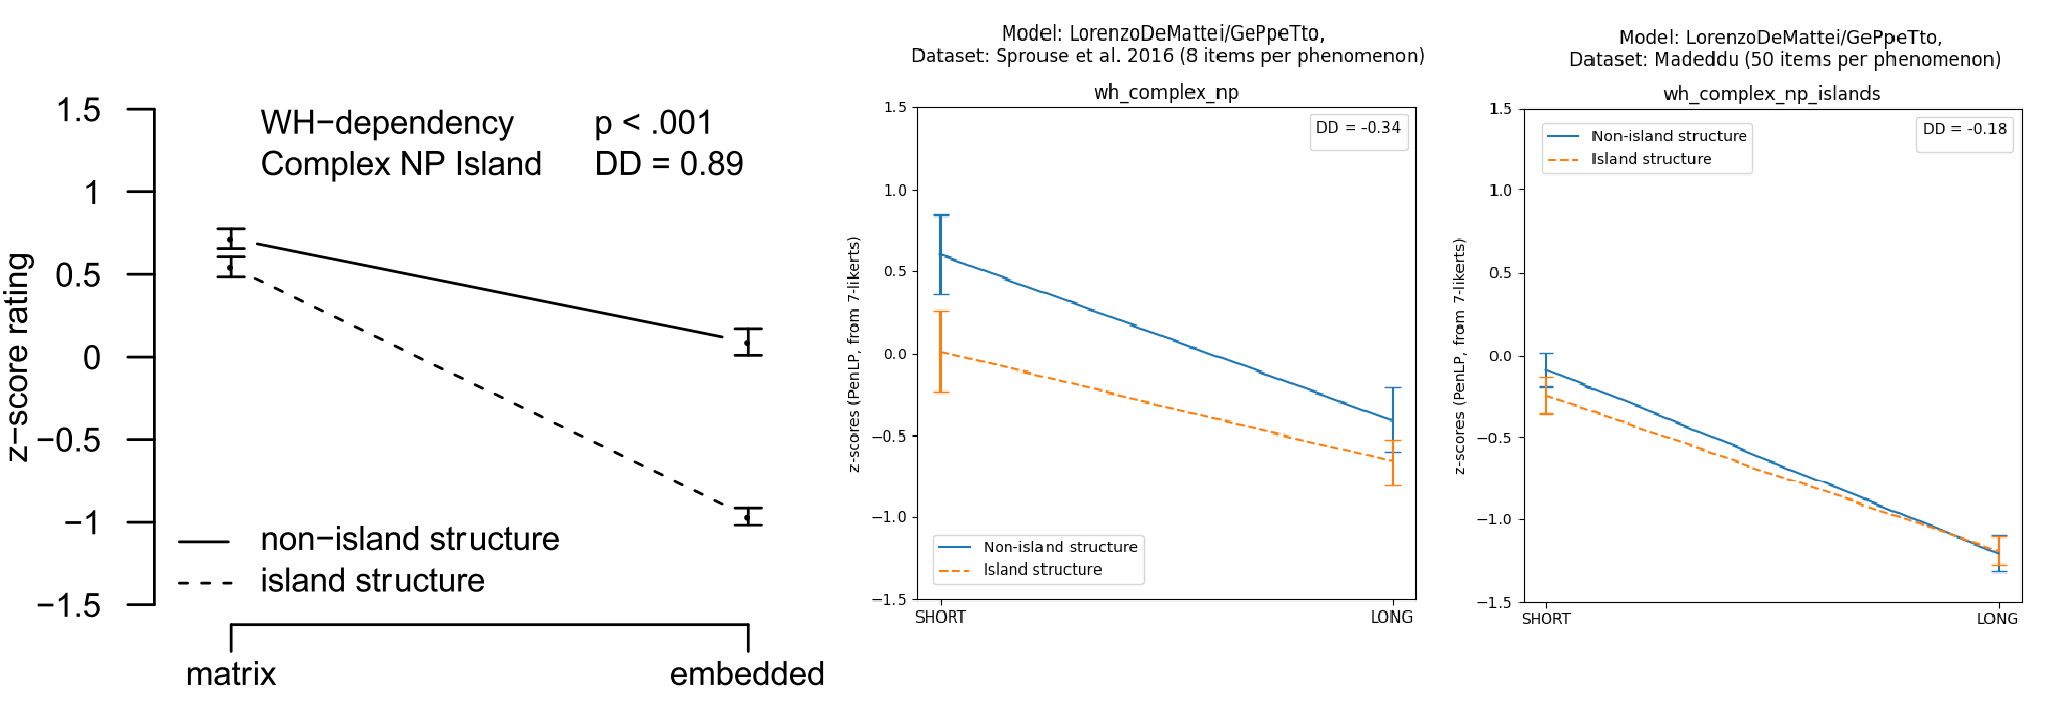
\includegraphics[width=1\textwidth]{images/Chapter1/combined_wh-complex.png} 
	\caption{Comparison of plots for wh-dependencies complex NP islands} 
	\label{fig:wh_complex} % this internally labels the figure for future referencing.
	\medskip
	\small
	The first plot on the left shows the scores on humans subjects published in \citet{sprouse2016experimental} for Italian complex NP islands with wh-dependencies. For each line, the left-most edge represents the score for the short-distance dependency sentence, the right-most the long-distance dependency. The plot in the middle shows the scores from a Gpt-2 model \citep{de2020geppetto} on the same test suite used for the first plot. The plot on the right shows the scores from the same Gpt-2 model but on the expanded test suite developed for the present thesis.
\end{figure}

Doing some variations experiments (see  \autoref{tab:compare1}), we found that by replacing the main clause verbs with "intuire che"/"avere l'intuizione che" ("to sense that" / "to have the intuition that") or "avvertire che"/"avere il sentore che" ("to feel that" / "to have an inkling that") or "percepire che"/"avere la percezione che" ("feel that"/"to have the feeling that"), the island restriction violation seem to have no effect, and the Long-Island sentence becomes more acceptable than the same sentence without the island structure (Long-NonIsland).
 
Indeed, the sentence \textit{Cosa hai avuto l'intuizione che il portavoce avrebbe confermato?} (\textit{`What did you have the intuition that the spokeperson had confirmed?'}), seems acceptable despite extracting from a complex NP construct. 

An hypothesis, whose demonstration we leave for future work, is that this is due to main clause expressions in which the subject has the semantic role of an \textsc{experiencer} rather than an \textsc{agent}, which could be a condition for Complex NP island restrictions to enter into effect or not. 
% "avrebbe ppt" (condizionale passato)
% In fact, it seems that the Gpt-2 model correctly captures the fact that with these constructs the long nonisland sentences become acceptable.

\begin{table} \scriptsize 
	\begin{center}
		\begin{tabular}
			{p{0.3\linewidth} p{0.08\linewidth} p{0.3\linewidth} p{0.08\linewidth} p{0.08\linewidth}|} \\
			\multicolumn{2}{c}{\textbf{\textsc{Long-NonIsland}}} & \multicolumn{2}{c}{\textbf{\textsc{Long-Island}}}  &   \\
			\textbf{text} & \textbf{PenLP} & \textbf{text} & \textbf{PenLP} &  \textbf{Diff}  \\
			\hline
			\textit{Cosa hai messo in dubbio che il portavoce avrebbe confermato?} & -31.65
			& \textit{Cosa hai messo in dubbio la previsione che il portavoce avrebbe confermato} & -33.21 & 1.56 \\ 
			\textit{Cosa hai intuito che il portavoce avrebbe confermato?} & -32.36 
			& \textit{Cosa hai avuto l'intuizione che il portavoce avrebbe confermato?} & -29.99 & -2.37 \\ 	
			% TODO: use the other verbs too:  "avvertire che"/"avere il sentore che" ,  "percepire che"/"avere la percezione che" 
			\textit{Cosa hai detto che Gianni avrebbe sollevato?} & -33.74 
			& \textit{Cosa hai riferito il fatto che Gianni avrebbe sollevato?} & -36.64 & 2.90 \\ 
			\textit{Cosa hai intuito che Gianni avrebbe sollevato?} & -34.31 
			& \textit{Cosa hai avuto l'intuizione che Gianni avrebbe sollevato?} & -30.52  & -3.79 \\ 
			
			\textit{Cosa hai messo in dubbio che io avrei vinto?} & -26.48 & 
			\textit{Cosa hai messo in dubbio la previsione che io avrei vinto?} & -30.17 & 3.69\\ 				
			\textit{Cosa hai intuito che che io avrei vinto?} & -29.49 & 
			\textit{Cosa hai avuto l'intuizione che io avrei vinto?} & -24.45  & -5.04 \\ 				

		\end{tabular}
		\caption{Comparing acceptability variations among sentences in the complex NP dataset. A positive difference indicates that the Long-NonIsland sentence is more acceptable than the Long-NonIsland one, as expected.}
		\label{tab:compare1}
	\end{center}
\end{table}


\bigskip
% TODO: insert plot of variations
With other variations experiments, we found that replacing the main clause verb with "sapeva che"/"conosceva che" ("he knew that", see examples in table ..TODO), increases the acceptability of the long-non island sentences; on the other hand, this variation results in a lower acceptability to the short island sentence, compared to the scores from human subjects, and by this way the non-island and island line end up being almost parallel, with the DD score close to zero (which indicates an almost absent island effect).
\\ TODO: add table and plots of senteces with  "sapeva che"/"conosceva che" 
% todo: show tables with examples "sapeva che" % todo: numbered examples like formulas
% todo: show the plots for "intuizione che", "sapeva che" (two subfigures, each numbered/lettered to be referenced)

% examples of complex np items before and after the "avuto l'intuizione che" variation: ..
% show the plots for the items using this construct ("avuto l'intuizione che" ), it seems strange scores are given
% (the island line is higher than the non island one, but they are all acceptable sentence and there is no island restriction anymore)

% still the problem overall in the orginal plots seems an overly low score for the long non island sentences
% that is, is the long distance depencency that receives a too loo score .. (lenght effect?)
% while the structure effect ..
% albeit it's correct, like humans scores, that the long non island has less acceptability than the short island
% then how is the long distance dependency (lenght effect) scored for the other island phenomena?
% the difference with the sentences for the other phenomena seem to be that they have a simpler main clause, like "cosa pensi che" (present) + "abbia ppt"  (congiuntivo passato), while for the complex np, is "cosa hai smentito/annunciato/raccontato/sostenuto che" (passato prossimo) + "avrebbe ppt" (condizionale passato)
% a comparison example could be to turn the other 3 island phenomena items into passato prossimo for the main clause
% but was this discrepancy also in Sprouse data, and is this the reason for their plots differences too? (so the gpt2 model just accentuates this drop in acceptability?)

% for future work: automatic generation of examples from templates, like in BLiMP, to control and test more easily for more factors (es. verbs moods and tenses)
% to test for frequency effect: use some rare verb moods/tenses?

% also find an explanation for the other misclassified long non island sentences that use other constructus (with proper agent/patient semantic roles)

% table..

% Mostra una non robustezza del modello nell’apprendimento di strutture sintattiche / or of this use for scoring minimal pairs, non generalizzazione sintattica, in quanto basta una variazione lessicale, anche tra ..parole frequenti, ..per ..alterare ..quale tra due frasi coppie minime sia piu o meno accettabile.
% However, we refer back to section .., about the interpretation/meaning of the Gpt-2 loss ..output/score.


% TODO: table with example items with different constructs, and their scores
% TODO: plots of the whole test suite for this phenomenon with the same variation for all items (using a different verb)



\subsubsection{Whether islands}

From \autoref{fig:wh_whether} for whether islands with wh-dependencies, we can see that the Gtp-2 model, with the PenLP sentence acceptability estimate, compared with the results from humans gives higher scores for all sentence types. This difference is more pronounced in the scores performed by Gpt on the original test suite from \citet{sprouse2016experimental} (middle image). 

The slope of the lines (both for island and non-island sentence structures) is however quite similar to the human scores. \\


\begin{figure}[H]
	\centering
	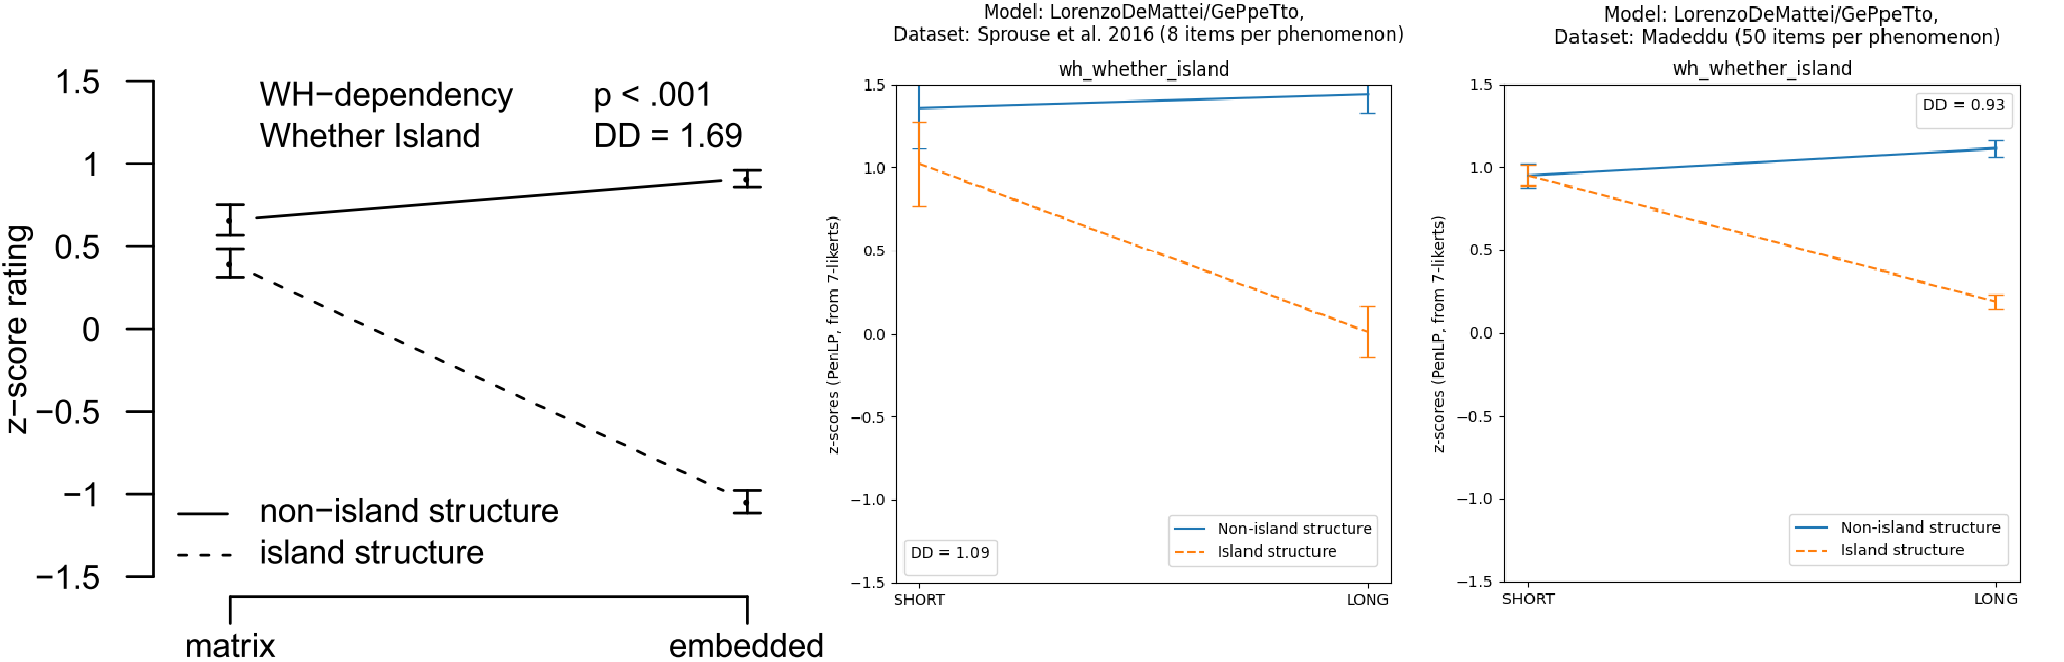
\includegraphics[width=1\textwidth]{images/Chapter1/combined_wh-whether.png} % width= 0.8\textwidth
	\caption{Comparison of wh-dependency whether islands} 
	\label{fig:wh_whether} % this internally labels the figure for future referencing.
\end{figure}

..

% TODO: table showing accuracy scores for the 4 sentences of an item; comparison on variations across multiple items

Experimenting with other sentence variations for whether islands, we found that a variation that aligns the plots more to those from the humans' scores, is replacing the personal pronouns (like "io") with proper nouns (like "Gianni") or common nouns (like “il parlamentare”, or “lo studente”)  like in this example: 

\begin{example}	\textsc{Whether islands, Long-Island sentence type}
	\renewcommand{\labelenumi}{\alph{enumi}.}
	\begin{enumerate}
		\item 
		Cosa ti domandi se io abbia riscosso?
		\item 
		Cosa ti domandi se Gianni abbia riscosso?
		\item 
		Cosa ti domandi se il parlamentare abbia riscosso?
	\end{enumerate}
	\label{variation_2}
\end{example}

% This might be the reason for the discrepancies in some of the 4 phenomena: some make more use of ..nomen agentis, while others rely more on personal pronuns. Try this replacement this in all 4 test sets.
TODO: put scores values and/or to quantify the effect of these variations.

TODO: test sentence variations using less common verb tenses and moods  % Not much difference seems to derive by using less common (..) verbs
% (examples in which both sentences in a pair also specify the direct object, see how this affects the score? Like long nonisland vs long island ..)


\subsubsection{Subject islands}

\begin{figure}[H]
	\centering
	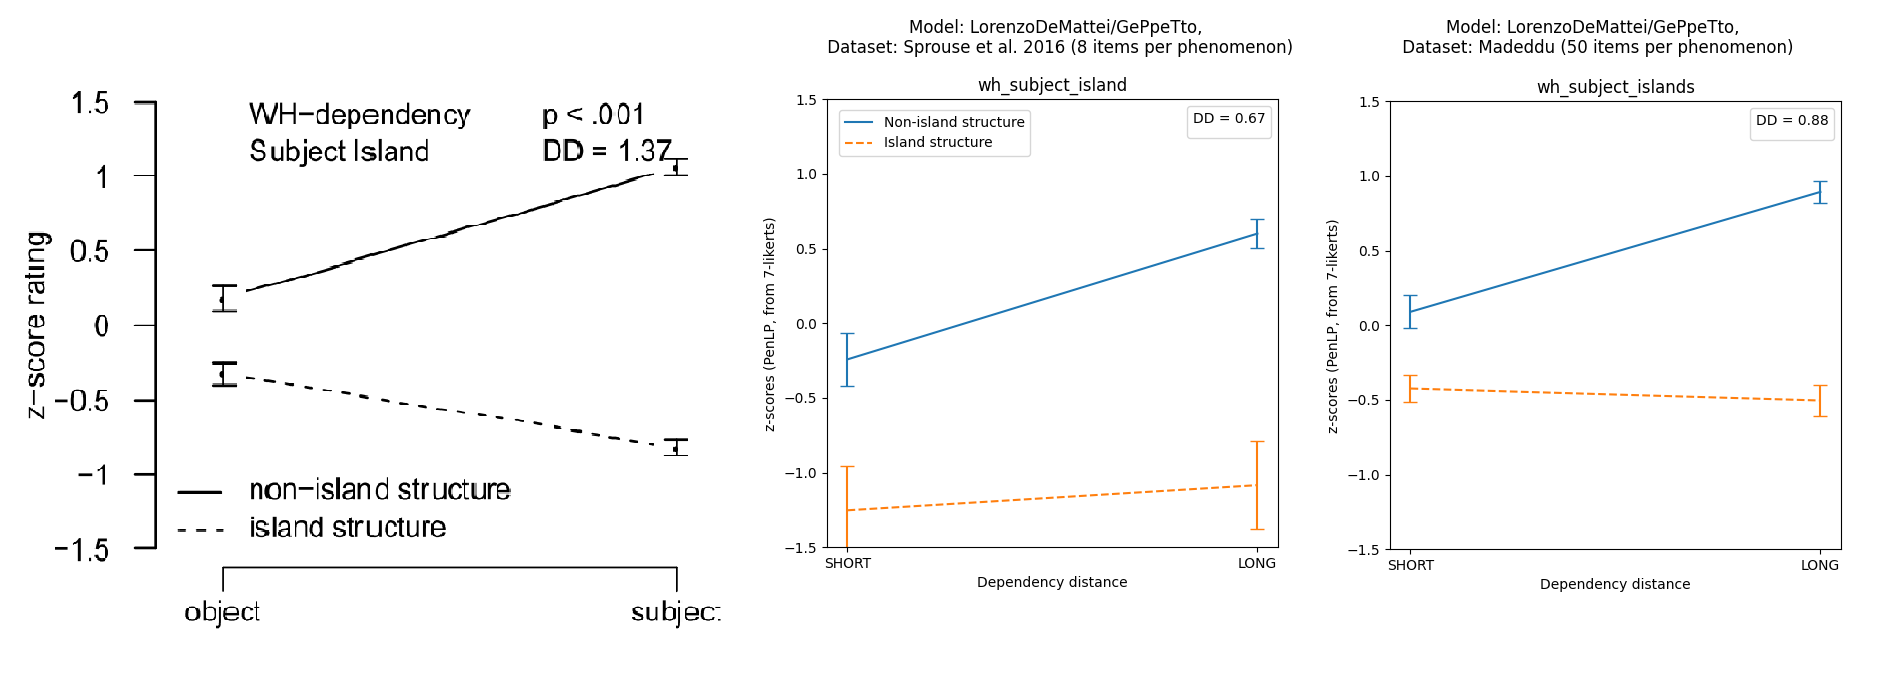
\includegraphics[width=1\textwidth]{images/Chapter1/combined_wh-subject.png} 
	\caption{Comparison of wh-dependencies subject islands} 
	\label{fig:wh_subject} % this internally labels the figure for future referencing.
\end{figure}

In \autoref{fig:wh_subject}, the middle image of Gpt scores on Sprouse data shows significantly lower scores (compared to the human scores on the left image) for the sentences with an island structure (dotted line). % check the sorting of sentences to see why). 
However, on the right image (Gpt scores on our test suite) they are similar to the human scores. \\

For the non island line, the Short-NonIsland is scored lower then on human subject by Gpt for both testsuites. The Long-NonIsland scores instead are similar  (around 1.0). % but lower on sprouse data. \\
The slope of the lines on the right image is similar to the one for the human scores (left image). %  oneon the model scores, both for sprouse and new data, but steeper compared to acceptability results on human subjects.


\subsubsection{Adjunct islands}

\begin{figure}[H]
	\centering
	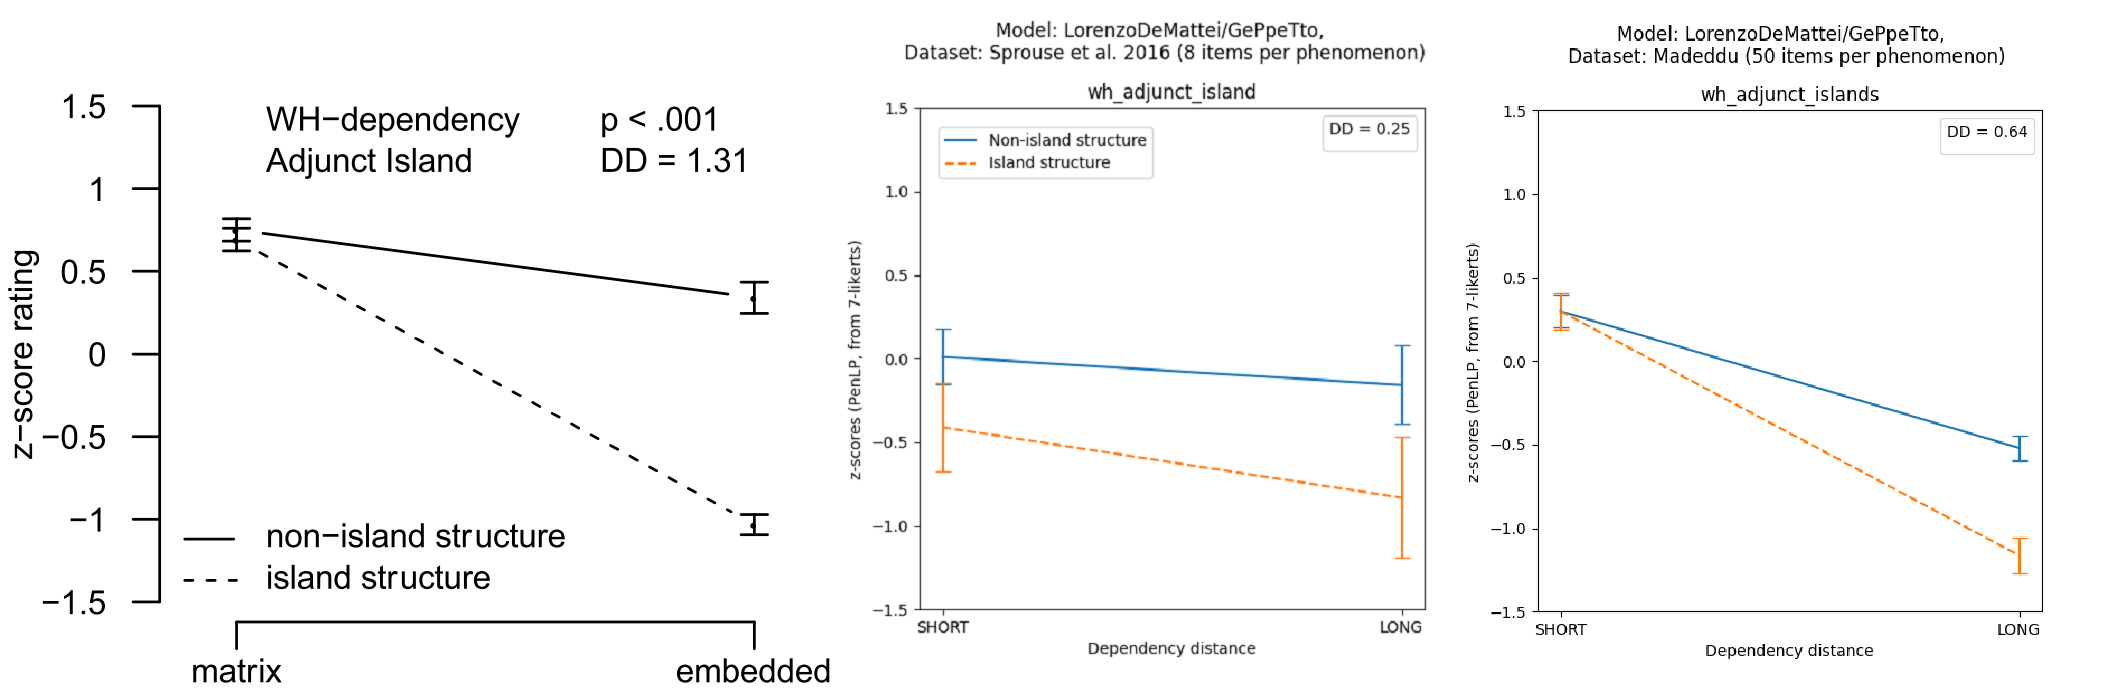
\includegraphics[width=1\textwidth]{images/Chapter1/combined_wh-adjunct.png} 
	\caption{Comparison of wh-dependencies adjunct islands} 
	\label{fig:wh_adjunct} % this internally labels the figure for future referencing.
\end{figure}


In \autoref{fig:wh_adjunct} the slope of both lines on the new test suite (right image) is similar to the human scores (left image), althoughg with a lower average acceptability for the Long-NonIsland sentences, which results in a downward steeper line. 

Note that in the test suite we developed for this thesis, the Long-Island sentences for adjunct islands have a form that might make them more easily identifiable has unacceptable than the ones in the Sprouse test suite: compare \textit{Che cosa Gianni è partito per Parigi dopo aver fatto?} (new dataset) with \textit{Cosa ti irriti se dimentico in ufficio?}. The ending of the first sentence might be less frequent and result in a lower acceptability score.
% in the sprouse data, at the end there is a preprositional ..phrase like “in ufficio”.


\subsubsection{Overall observations across all four island phenomena}

The Gpt-2 scores on the original Sprouse et al. test suite (middle image) have wider standard error bars, which are considerably smaller for the new test suite developed for the present thesis (right image).\footnote{This might be due to the fact that the number of items between the two test suites increases from 8 to 50.}


While on human ratings the unacceptable sentences (Long-NonIslands) receive all on average a z-score of about -1, there is more variability in the scores given by the Gpt model, in particular for whether islands sentences (\autoref{fig:wh_whether}), which receive much higher acceptability rating on average (betwenn 0 and 0.5 the Sprouse test suite and ours).
..

% TODO: remaining tables with accuracy scores, comparison with BLiMP extraction islands scores; compare btw models, scoring measures, and datasets (BLiMP, Sprouse, Madeddu)

% todo: all the plots in the appendix (BERT, LP/PenLP, logistic LP/PenLP, .. ) and brief comments 
% (like limitations of BERT acceptability estimates)

% Italian models:
% "LorenzoDeMattei/GePpeTto"
% "dbmdz/bert-base-italian-xxl-cased": ModelTypes.BERT,
% "idb-ita/gilberto-uncased-from-camembert"

% testsuites/datasources:
% Sprouse et al.
% Madeddu

% scoring measures:
% LP/PenLP (softmax-based)
% % LP/PenLP (logistic-based)


\subsection{Discussion on plots from BERT, the logistic function, and PenLP}

% BERT-like models, LP/PenLP scores also based on logistic function scores
% (comment also on the accuracy scores from other models?)

In \autoref{fig:bert_penlp_l_sprouse} we see the plots of the scores from the BERT model, with the PenLP-L sentence acceptability estimate (using the logistic function rather than the softmax, as described in \autoref{sec:softmax}). Interestingly, it seems that this combination of BERT with the logistic function makes a clear separation between unacceptable sentences (the Long-NonIsland type) and acceptable sentence types, with minimal, if any, difference in score between acceptable sentences.

\begin{figure}[H]
	\centering
	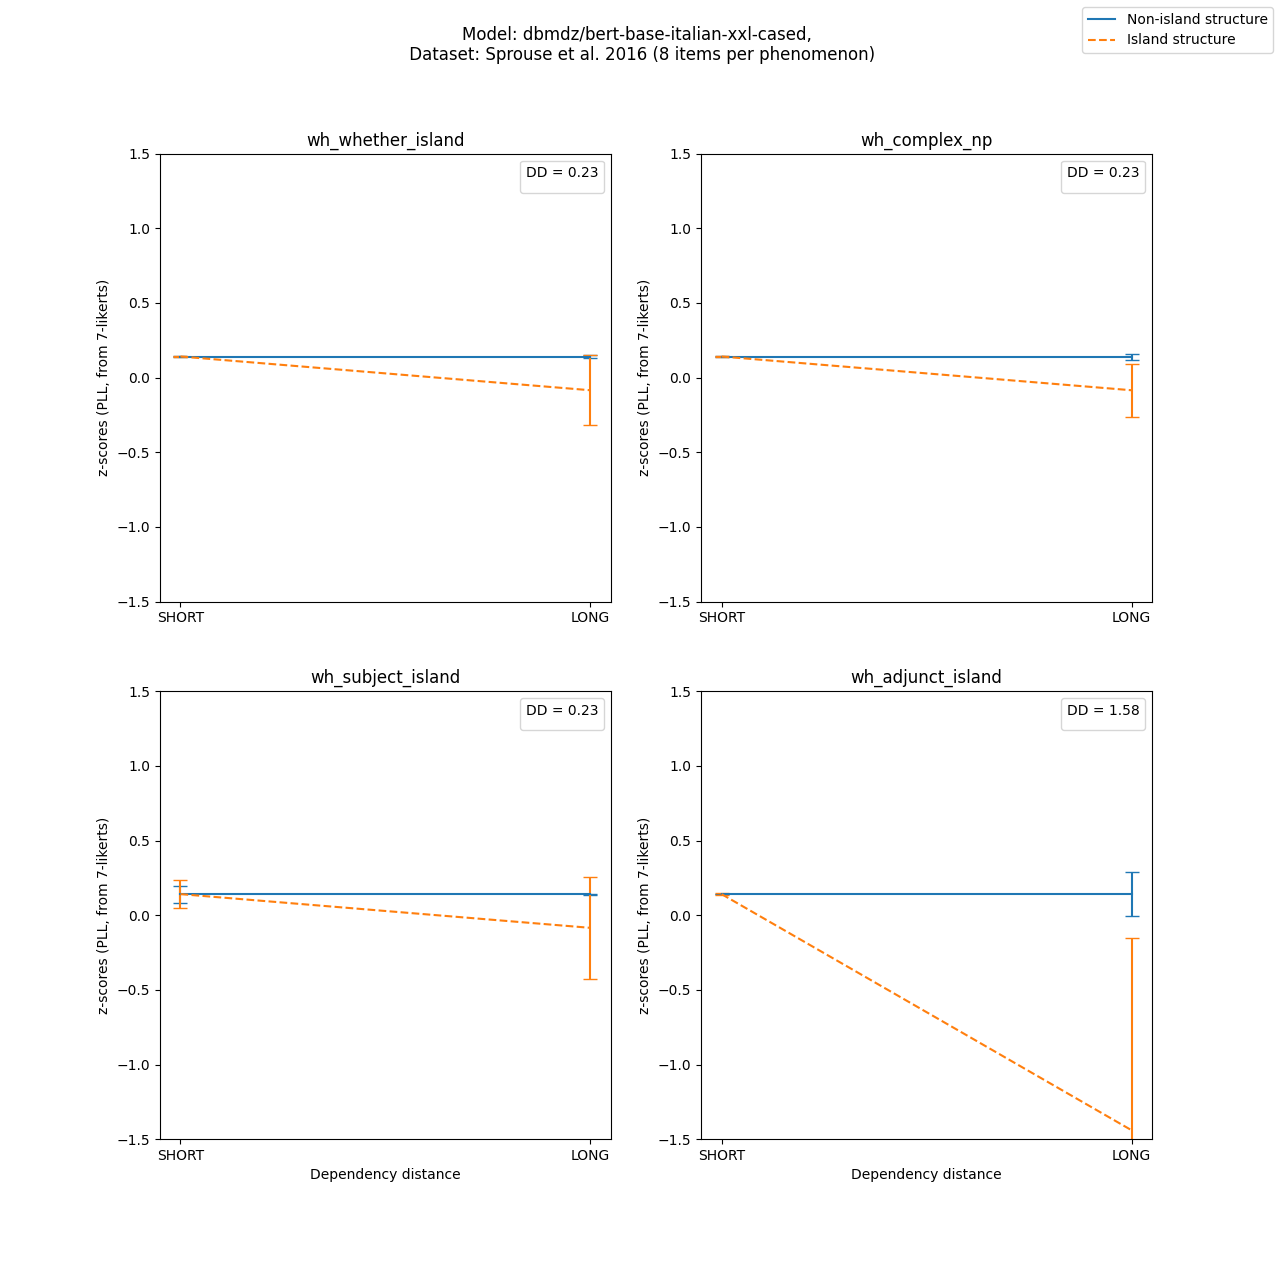
\includegraphics[width=1\textwidth]{images/AppendixA/Sprouse_wh_dbmdz_bert-base-italian-xxl-cased_PLL-zscores-likert-2022-07-11.png} 
	\caption{Plots from BERT with the PenLP-L sentence acceptability approximation}
	\label{fig:bert_penlp_l_sprouse}
\end{figure}

If we compare these plots with the accuracy scores in \autoref{tab:accuracy_it_data} from this model (BERT, logistic function, PenLP) , we see that they are among the best with an average accuracy of 80.7\%; however, looking at the scores for each phenomenon, the scores are high only in about half the cases, and quite low for the rest: Long-NonIsland sentences of all four island phenomena are scored with 58\%, 64\%, 74\%, 58\% accuracy, and the Short-NonIsland of subject islands with 28\% accuracy.

TODO: check if this is also a skewing effect of the normalization (from the likert scale and the z-scores) and the presence of much negative large values for the unacceptable sentences: in this case the normalization would ..squeeze together the score for the acceptable sentences, if they have a smaller magnitude.

% With the , the use of the logistic function scores as a basis for LP/PenLP instead results in much ..worse plots (  ). Whether, complex and subject islands get almost identical plots, due to the ..skewing/normalization effect of the discretization and the zscores, because the adjunct islands have much higher magnitude negative values (low acceptability) for the unacceptable sentence (long island.) (? so it seems that with BERT and logistic function scores emerge more clearly a distinction between acceptable and unacceptable sentences, without much differenciation within these two groups).

\subsection{Discussion on plots from GilBERTo}

Overall, for GilBERTo, the plots are significantly different from those on human ratings. (..)

\begin{figure}[H]
	\centering
	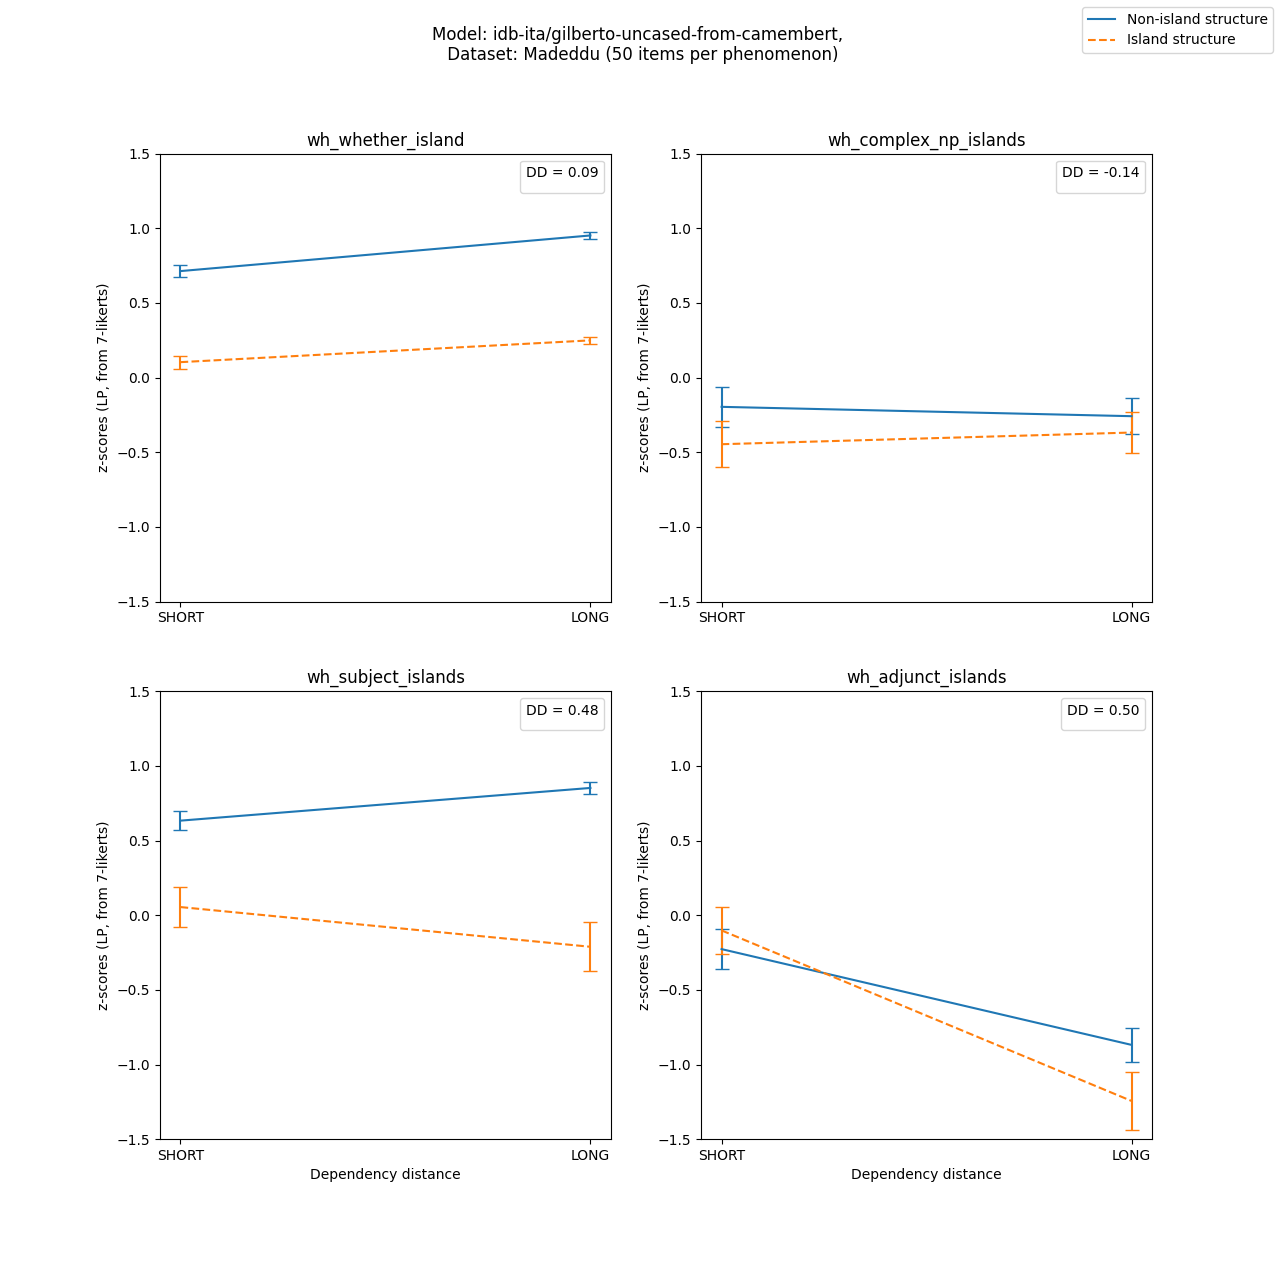
\includegraphics[width=1\textwidth]{images/AppendixA/Madeddu_wh_idb-ita_gilberto-uncased-from-camembert_LP-zscores-likert-2022-07-11.png} 
	\caption{Plots from GilBERTo with the LP sentence acceptability approximation}
	\label{fig:gilberto_lp_madeddu}
\end{figure}

\section{Drafts}
\subsection{Observation on plots for other models}


The plots for Geppetto and PenLp are the most similar to the plots on human ratings. However, with the LP measure, the plots differ significantly.

The plots for BERT with PenLP on the Sprouse data are similar to the results on humans from \citet{sprouse2016experimental}, ..with some ..differences..


In the plots from the GilBERTo scores, we see that for complex NP and subject islands, the sentences with the island structure receive a higher acceptability than the non island ones (this is no longer the case when removing the penalty for sentence lenght, using the LP sentence acceptability measure). With the PenLP sentence acceptability approximation, the lines tend to have similar slopes, close to being parallel (indicating a lack of, or small, island effect). 


Plots on the Madeddu dataset developed for the present thesis:

BERT, softmax, PenLP and LP
..
for adjunct islands, LP seem to work best (without penalizing for sentence lenght).
Using the logistic function scores, again we see the ..binary differentiation btween unacceptable (long non island) and acceptable (the other 3 types) sentences. However here the plots are more ..flattened, with the scores being very close to the same values.

We refer to the Appendix for the plots for the other models.

\subsection{What seems to affect the models acceptability scores}


\subsubsection{Adjunct islands}

Guardando le short-nonislands, sembra anche qui preponderante il fatto di usare nomi propri di persona (che ha uno score di accettabilità minore) e usare invece di nomi comuni animati/di mestieri/.. (che aumenta l’accettabilità). Ma questo non sembra influenzare il DD score finale (..evidentemente i vari fattori si bilanciano).


\subsection{Discarded observations on differences between the plots}

\subsubsection{Other notes on  Complex np islands,  what seems to affect the models acceptability scores}
In \autoref{fig:wh_complex} we see that the non-island line (the line connecting the two acceptability scores for short and long distance dependency sentences without an island structure) is significantly lower in new data (todo: see constructs that increase the score of both long and short)

The (gpt) model seem not to make much difference in ..acceptability btw “regular” subordinates and complex noun phrases ..

-- also the short island point is significantly lower

All the 50 + 8 items of the two test suites (the ones from Sprouse et al and the ones developed for the present thesis), when altered to use the following construct for the complex NP "avuto l'intuizione che" (had the intuition that), are scored by the model as if there is no island restriction violation anymore. 

il verbo “intuire” diminuisce ..l’accuratezza del giudizio di accettabilità
in particolare diminuzione della accettabilità delle frasi long nonisland (con long distance wh dependency e struttura non island), che ricevono accettabilità minore di quelle con struttura island:
Esempio analisi variazioni con verbo “intuire” complex np, ..

the verb form “sapeva” (imperfect), compared to ..present perfect forms (“ha osservato/affermato/..”) seems to get better DD score in complex np islands (and also in another phenomenon ..).

\subsubsection{Whether islands}
NB: note that according to human scores, for this type of whether island sentences, the "correct" scoring is to have an increase in acceptability going from short to long non island sentences.
Maybe comparing the scores between acceptable sentences (in this case short and long non islands), expecting it to match humans acceptability judgements .. is beside the present ..research question.
In any case, we noted a reverse in the acceptability difference between this two types of sentences (short and long non islands) when changing the subject of the subordinate sentence from a personal pronoun ("io", 1st pers sg), to a proper noun (i.e. "Gianni"), to a common noun (i.e. "il parlamentare").

-- significant variation in acceptability diff between short non island and long non island, when replacing: the personal pronouns io/lei, with a proper noun like "Gianni", or even more with a noun like "il parlamentare" (the congressman). In this latter case, significant improvement toward the expected acceptability rate (only 10 out of 50 are .."missclassified"). With the proper noun "Gianni", 18 are missclassified. With the personal pronoun 29 out of 50 are missclassified.
Try replacing with .. another proper noun, more common like ..


(tables and examples of these variations to put on the thesis/report?)

(possible explanation: personal pronouns and proper nouns might be less common in the type/genre of corpora these models were trained on, like wikipedia).
Observations: the direct objects in the examples are all relatively common words..\footnote{\citet{wei2021frequency} found significant frequency effects (but for agreement .. tests, which are much easier to isolate), for items that occurr rarely in the training corpus (..less then ..10-100 times). But to notice this effect they had to purposly tweak the training corpus. Replicating this for a preexisting corpus (using very rare vocabulary ..) is much more complex and out of the scope of the present study.}
try with rarer ones.
..
-- both on sprouse and new data, gpt "incorrectly" increases the accceptability from short to long non island (check constructs that instead decrease the acceptability?)

\subsection{Future work}
..
Analizzare le attivazioni nei vari livelli del modello ..
Fare un training .”a strati”, in cui in ciascuno strato c’è il target dell’apprendimento di un livello di base della lingua (morfologia, sintassi, semantica, ampiezza del vocabolario, ..), con strati successivi che aumentano la complessità della conoscenza che il modello ha del linguaggio.


Confronto percentuali accuratezza (short/long non island, short island) con quelle in BLiMP
(and other works with extraction islands evaluations?)


\section{BLiMP English dataset}
..
\subsection{English models details}
..
\section{misc ideas with notes}

..
(misc ideas with notes)
using multiple POS taggers and semantic role taggers etc.
one, the default, for most common (..more prototypical) sentences/structures
the other ones, used in ..garden path scenarios, when multiple indicators show that some POS tags or semantic role or other category might be wrong.
the second set of taggers should do a ..full parsing analysis.. combining and ranking different parsing hypotheses)


(on perplexity: the target of "low perplexity" in a language model, should not be in the ..words themselves, because language has informative/comunicative goals that are to introduce new, less predictable, information; it should be at other levels, like that of correctedness/acceptability; target of low perplexity of POS tags, semantic role tags, etc.) \\
\citet{von2018pos} use perplexity on POS tags as a measure of syntactic complexity;
"working on POS sequences avoids having to deal with data sparsity issues." \citep{von2018pos}

what about using perplexity on POS tags as a measure/estimation of syntactic well formedness?
": Lawrence et al. (2000) train RNNs to do
acceptability classification over sequences of POS
tags corresponding to example sentences from a
syntax textbook."

discriminate btw complex/rare vs unacceptable? a threshold (linearly separable) on perplexity? Or multiple dimensions, non linearly, should be used?
(but if there is a wrong/mispelled word.. the pos tagger might misclassify it)
(distinguishing ..sentence unacceptability by linguistic level: morphological mistakes/typos, ..word order errors, ..)
(also: perplexity uses a markov model of language? no, but multiplication the perplexity of each word to obtain the perplexity of the whole sequence.. a "less linear" formula might be needed..)
(montemagni et al paper on profileU on linguistic profiling? use for sentence acceptability estimates? use for ..style detection/automated analysis ..


\section{Misc notes with refs}



“NATURAL LANGUAGE DOES NOT MAXIMIZE PROBABILITY” 
“Why is human-written text not the most probable text? We conjecture that this is an intrinsic property of human language. Language models that assign probabilities one word at a time without a global model of the text will have trouble capturing this effect. Grice’s Maxims of Communication (Grice, 1975) show that people optimize against stating the obvious. Thus, making every word as predictable as possible will be disfavored. This makes solving the problem simply by training larger models or improving neural architectures using standard per-word learning objectives unlikely: such models are forced to favor the lowest common denominator, rather than informative language.” 
\citep{holtzman2019curious}

Repeated exposure to a type of island construct will increase its perceived acceptability 
\citep{chaves2014subject}

First work with targeted syntactic tests on modern language models (RNNs or transformers) is \citet{linzen2016assessing}, while first use of psycholinguistic tests for modern LM is from \citet{futrell2018rnns}.

"Auxiliary training objectives Adding auxiliary unsupervised training objectives is an alternative form of semi-supervised learning. Early work by Collobert and Weston [10] used a wide variety of auxiliary NLP tasks such as POS tagging, chunking, named entity recognition, and language modeling to improve semantic role labeling. More recently, Rei [50] added an auxiliary language modeling objective to their target task objective and demonstrated performance gains on sequence labeling tasks. Our experiments also use an auxiliary objective, but as we show, unsupervised pre-training already learns several linguistic aspects relevant to target tasks." (Radford Gpt)

"QUALITATIVE ANALYSIS" (REASONING ABOUT ENTAILMENT WITH NEURAL ATTENTION, Tim Rocktaschel et al. 2016)

"Efficiency considerations are important when building language models that use
such large sets of n-grams. Rather than store each word as a string, it is generally
represented in memory as a 64-bit hash number, with the words themselves stored
on disk. Probabilities are generally quantized using only 4-8 bits (instead of 8-byte floats), and n-grams are stored in reverse tries." (Jurafsky 2021 3rd ef ch.3)

"the standard information theory textbook Cover and Thomas (1991). "

\nocite{wei2021frequency, hu2020systematic, lau2020furiously, bostrom2020byte, futrell-etal-2019-neural}
